\section{Experiments}
\label{sec:experiments}

\subsection{Evaluation protocol}
\label{sec:setup}
The source-family comparison pairs ordinary and prefix-supervised checkpoints across eight scenes (Table~\ref{tab:sourcefilter}). We additionally test independent ordinary training runs on three scenes (Table~\ref{tab:ordrep}). For budget sweeps and matched adaptation, we use three prefix-supervised checkpoints per scene on four scenes: Chicken (HyperNeRF VRIG~\cite{park2021hypernerf}, 164 frames at $268\times480$), Cut Roasted Beef and Sear Steak (DyNeRF/N3DV~\cite{li2022neuralvideo}, 300 frames each at $480\times360$), and Basin (NeRF-DS~\cite{yan2023nerf}, 668 frames at $240\times135$). These scenes and test views had been examined previously. The independent runs quantify variation across training seeds within a scene.

For each source and nominal retained fraction, O, P, C and U have identical integer capacity $K$ and use identical test cameras. For the four-scene study we average raw PSNR over frames within each checkpoint, then report the scene mean and sample standard deviation over the three checkpoint values. Paired differences compare methods within each checkpoint before aggregation. All quality cells contain PSNR. Each auxiliary metric (SSIM and LPIPS) is missing for 46 archived Basin cells: ten at 10\% retention and twelve each at 15, 20 and 35\%. We leave these entries missing. The source-family comparison, within-scene repeats and supplemental 13-scene P/O study are reported separately.

\subsection{Ranking choice across source representations}\label{sec:sourcefamily}
We tested whether the benefit of restricting candidates changes with the source representation. We held the scene, camera sequence and retained fraction fixed, and compared C with U within each source. We used ordinary 4DGS checkpoints whose saved training configurations disabled prefix supervision. In addition to Chicken, Cut and Sear, we included all five additional real scenes with both an ordinary seed-zero checkpoint and a prefix-supervised source in the prepared-scene archive. These scenes had previously been examined under a different selection protocol. All low-budget comparisons used the same 50\% candidate pool and the same 32 training observations within scene. The comparison addresses transfer between existing sources. Training configurations and final point counts also differ between source families.
\begin{table}[!htbp]\centering\small
\caption{Effect of restricting the influence ranking to the more opaque half of the source. Entries give cold C minus U in mean test PSNR (dB). Both families use seed zero. Each difference compares equal point counts and identical frames within a trained source.}\label{tab:sourcefilter}
\begin{tabular}{lrrrr}\toprule
&\multicolumn{2}{c}{Prefix-supervised}&\multicolumn{2}{c}{Ordinary 4DGS}\\
Scene & 10\% & 15\% & 10\% & 15\% \\\midrule
Chicken & +0.528 & +0.074 & -1.742 & -2.830 \\
Cut Roasted Beef & +1.144 & +0.462 & -0.356 & -0.270 \\
Sear Steak & +0.923 & +0.386 & -0.191 & -0.101 \\
Coffee Martini & +1.092 & +0.521 & -0.356 & -0.720 \\
Flame Steak & +0.618 & +0.290 & -0.001 & -0.187 \\
Broom & +0.577 & +0.179 & -5.820 & -6.973 \\
3Dprinter & +0.120 & +0.032 & -1.966 & -2.937 \\
Peel Banana & +0.387 & +0.080 & -0.683 & -0.982 \\
\bottomrule\end{tabular}\end{table}
Across the eight paired seed-zero scenes in Table~\ref{tab:sourcefilter}, C exceeded U on every prefix-supervised source at both budgets. On ordinary Broom, restricting the candidate pool reduced PSNR by 5.820 and 6.973~dB at 10\% and 15\%, respectively. Appendix~\ref{sec:absolute} gives the native full counts and absolute full, O, C and U PSNR for every pair. U led on all eight ordinary sources at both budgets, with a near tie on Flame Steak at 10\%. On the ordinary Cut source at 10\%, U and C still exceeded opacity by 10.309 and 9.952~dB, respectively. The influence score remains useful on this source even though the filter reduces its benefit.


\runinheading{3}{Independent ordinary training runs.}
We repeated the comparison on three scenes selected from Table~\ref{tab:sourcefilter} to span different seed-zero gaps at 10\%: Broom (largest), Chicken (intermediate) and Flame Steak (smallest). These are within-scene training repeats. We evaluated an existing second Broom checkpoint and trained Chicken and Flame Steak from initialization with a second seed. Each run used the original ordinary scene configuration, 3,000 coarse and 30,000 fine updates, with prefix supervision disabled. The seed pairs shared prepared data, 32 training-only calibration observations, held-out frames and budget rules. Each checkpoint was evaluated at its own native count and at both fixed fractions. Table~\ref{tab:ordrep} gives individual paired effects; the public archive gives absolute full/O/C/U values and individual frame measurements.

\begin{table}[!htbp]\centering\small
\caption{Ordinary 4DGS training repeats. Each cell is U minus C in mean held-out frame PSNR (dB) for one independently trained checkpoint. Both orders retain exactly the same number of primitives within a cell.}\label{tab:ordrep}
\begin{tabular}{lrrrr}\toprule
 & \multicolumn{2}{c}{10\% retention} & \multicolumn{2}{c}{15\% retention}\\
Scene & Seed 0 & Seed 1 & Seed 0 & Seed 1 \\\midrule
Broom & +5.820 & +4.211 & +6.973 & +4.923 \\
Chicken & +1.742 & +2.097 & +2.830 & +3.351 \\
Flame Steak & +0.001 & +0.770 & +0.187 & +1.072 \\
\bottomrule\end{tabular}\end{table}
For the second ordinary Broom, Chicken and Flame Steak sources, U minus C was +4.211, +2.097 and +0.770~dB at 10\% retention, respectively. At 15\%, the corresponding differences were +4.923, +3.351 and +1.072~dB.

Figure~\ref{fig:broom10} shows where the loss occurs on a held-out frame. C breaks up the continuous pavement around the broom and introduces high-contrast streaks across the ground. U recovers the pavement boundary and broom silhouette, although the bristles and fine pavement texture remain softer than the reference. The whole-frame PSNR is 12.74~dB for C, 19.06~dB for U and 23.11~dB for the full source.
\begin{figure}[!htbp]\centering
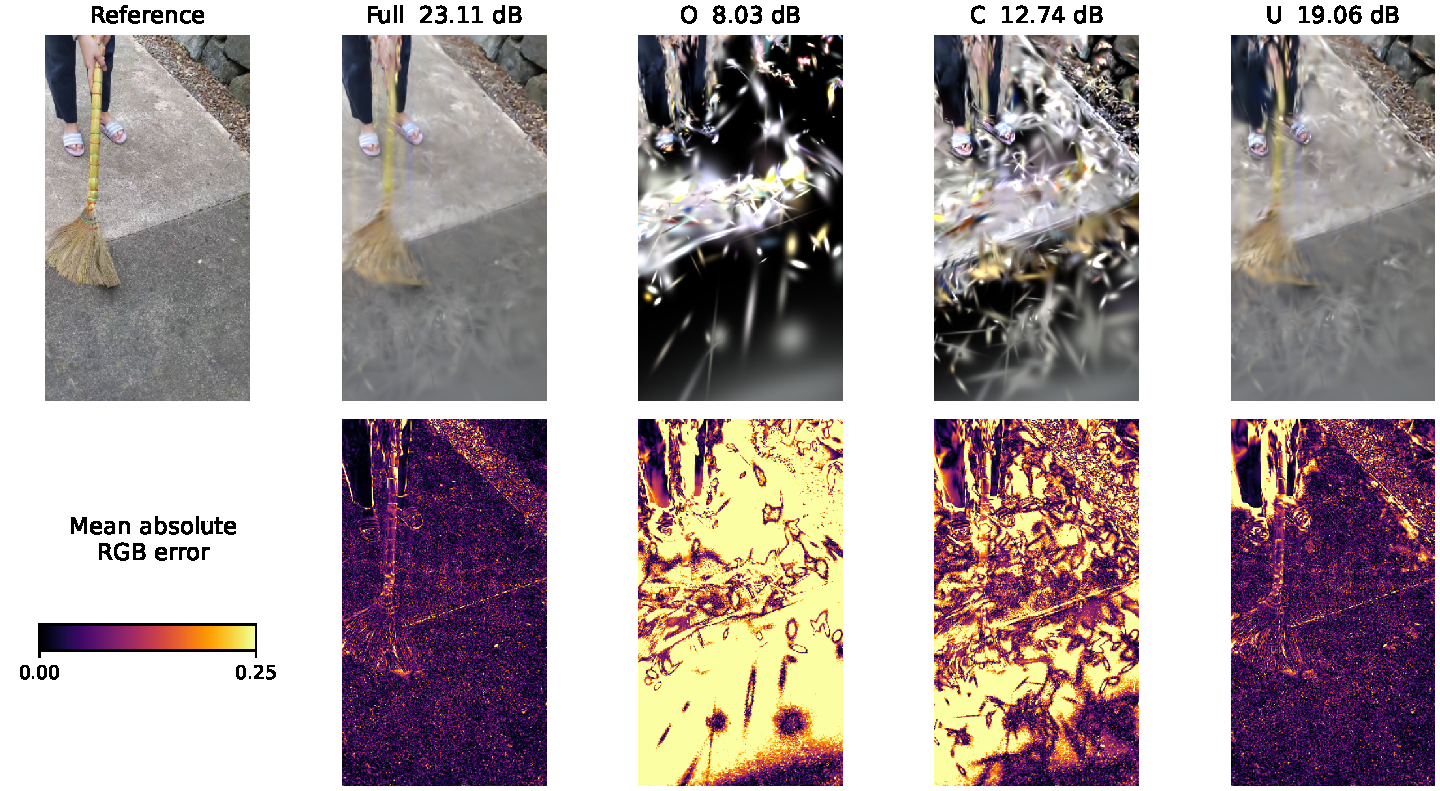
\includegraphics[width=\linewidth]{broom_10.pdf}
\caption{Ordinary Broom at 10\% retention (seed zero, 7,886 of 78,863 points). From left to right: reference image, full source, opacity (O), restricted influence (C) and unrestricted influence (U). Each label is whole-frame PSNR against the reference. The lower row shows mean absolute RGB error on the same linear scale, clipped at 0.25 on $[0,1]$ images. We chose the middle of the 197 held-out frames by list position (zero-based index 98), independently of frame quality.}\label{fig:broom10}\end{figure}


\subsection{Budget dependence before fine-tuning}
\label{sec:cold}
Table~\ref{tab:cold} and Fig.~\ref{fig:budget} report the same 240 quality cells across five budgets. At 10\%, C improves on opacity ranking (O) by 5.14~dB on Chicken, 2.26~dB on Cut and 1.55~dB on Sear, with improvements above 1~dB for every checkpoint from those three scenes. The respective differences at 15\% are 2.35, 1.85 and 1.06~dB, and at 20\% they narrow to 1.35, 1.45 and 0.76~dB. Basin has a smaller response throughout, with 0.11 and 0.09~dB gains at 10 and 15\%. The absolute values show that the small Basin gain occurs around 19.5~dB in this evaluation.

Comparing C with U isolates the opacity candidate restriction for the same analytic score. At both 10 and 15\%, C scores higher for all nine checkpoints from Chicken, Cut and Sear. At 20\%, C is ahead for two of nine checkpoints, and at 25 and 35\%, U is ahead for all nine. Basin differences between these variants are negligible. P and O select the same members at 10\% because P protects the opacity core at that budget. Additional 25\% controls hold the protected core and candidate band fixed (Table~\ref{tab:scorebridge}).

\begin{table*}[t]
\centering\small
\caption{Cold PSNR (dB), mean $\pm$ sample standard deviation across the three source checkpoints per scene. All four arms share the same sources, test frames and retained count for each budget.}
\label{tab:cold}
\resizebox{\linewidth}{!}{%
\begin{tabular}{lrcccc}
\hline
Scene & Budget (\%) & O & P & C & U \\
\hline
\resultrows{results_assets/cold.tex}
\hline
\end{tabular}}
\end{table*}

\begin{figure*}[t]
\centering
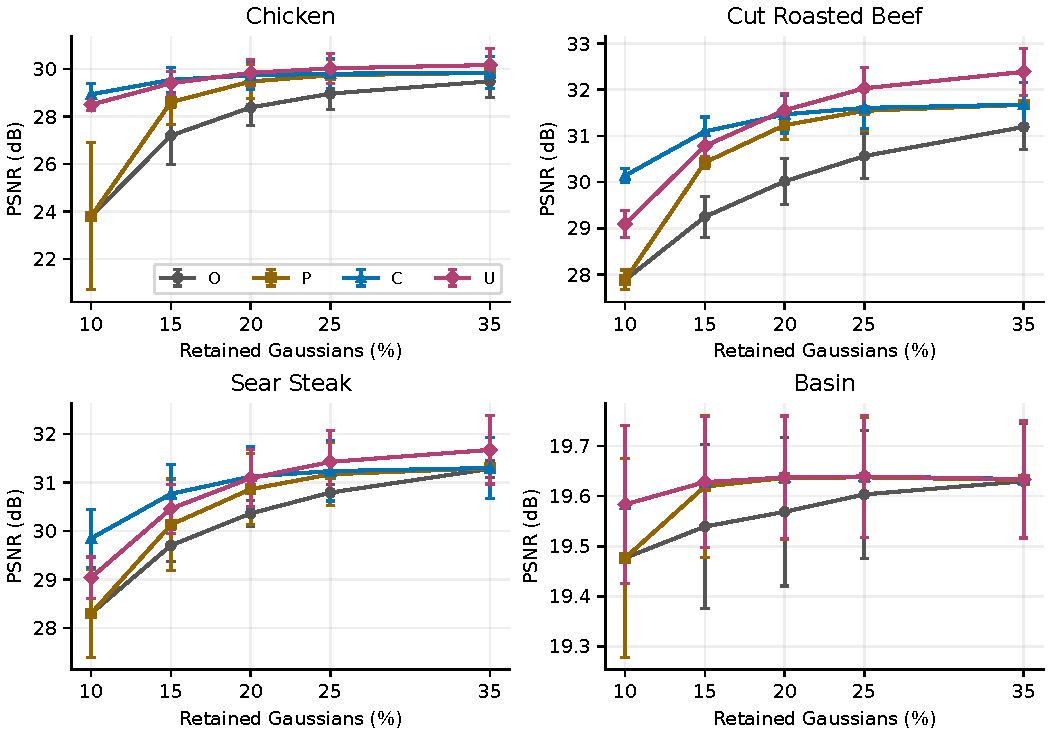
\includegraphics[width=.86\textwidth]{results_assets/budget.pdf}
\caption{Cold PSNR by retained fraction using the measurements in Table~\ref{tab:cold}. Error bars show one sample standard deviation across three checkpoints. The vertical scale varies by scene.}
\label{fig:budget}
\end{figure*}

\subsection{Ranking choice after matched fine-tuning at 15\%}
\label{sec:finetune}
For every source and ranking, we materialize the selected members at 15\% and apply 2,000 optimizer updates using common optimizer settings and the same training-camera schedule. Each run uses Adam to minimize $0.8L_1+0.2(1-\mathrm{SSIM})$ on training images, updating the retained point parameters and trainable deformation parameters. The endpoint is fixed in advance and test PSNR plays no part in choosing it. The membership remains fixed, with densification and member replacement disabled. The step-zero evaluations reproduce the archived cold per-frame PSNR with a maximum absolute deviation of $7.11\times10^{-15}$~dB. Table~\ref{tab:finetune} reports the fixed step-2,000 endpoint. Opacity subsets also benefit from the matched adaptation. The C--O gap remains positive for every Chicken, Cut and Sear checkpoint and exceeds 1~dB in all six Chicken and Cut pairs. U--O is negative for one Sear checkpoint ($-0.03$~dB), despite a positive scene mean. After fine-tuning, U exceeds C for eight of the nine Chicken, Cut and Sear checkpoints. P is below C for all nine. In Table~\ref{tab:finetune}, paired U minus C averages $+0.171$~dB on Chicken and $+0.566$~dB on Cut. On Sear the mean is $+0.002$~dB; its paired sample standard deviation, $0.452$~dB, reflects opposing changes across seeds. On Basin the mean difference is below 0.001~dB. Each adapted checkpoint serves its own 15\% working point.

\begin{table*}[t]
\centering\small
\caption{Matched fine-tuning at 15\%, PSNR (dB). Each entry is a mean $\pm$ sample standard deviation over three source checkpoints. The last column summarizes within-checkpoint differences.}
\label{tab:finetune}
\resizebox{\linewidth}{!}{%
\begin{tabular}{lccccc}
\hline
Scene & O & P & C & U & U--C \\
\hline
\resultrows{results_assets/finetune.tex}
\hline
\end{tabular}}
\end{table*}

\subsection{Candidate-pool width and repeated scoring}\label{sec:reschedule}
We then tested how much one-pass ranking loses when the compositing context changes. On each of the three prefix-supervised Cut sources, the unrestricted four-pass comparator rescored the survivors after retaining 60\%, 35\%, and 20\% of the full set. The final scoring pass supplied both target counts. This adapts the iterative re-quantification principle of GaussianPOP to a shared fixed-count schedule. No optimizer updates were applied. The same camera--time observations were used on every pass.
\begin{table}[!htbp]\centering\small
\caption{Cut Roasted Beef, three prefix-supervised sources. Mean $\pm$ sample SD over three sources for PSNR and offline preparation time on the RTX 3090. Time includes scoring, ordering and intermediate subset formation after warm-up, with model and cameras resident. Peak PyTorch allocation averaged 578.4~MiB for each scored variant. Single-pass pool variants share the full-source scoring measurement.}\label{tab:rescore}
\begin{tabular}{lrrr}\toprule
Selection & 10\% (dB) & 15\% (dB) & Prep. (s) \\\midrule
Opacity & $27.882\pm0.216$ & $29.250\pm0.440$ & --- \\
One pass, 30\% pool & $30.332\pm0.378$ & $30.816\pm0.489$ & $0.544\pm0.002$ \\
One pass, 50\% pool & $30.141\pm0.152$ & $31.097\pm0.313$ & $0.593\pm0.037$ \\
One pass, 70\% pool & $29.277\pm0.244$ & $30.868\pm0.246$ & $0.552\pm0.003$ \\
One pass, all candidates & $29.093\pm0.286$ & $30.782\pm0.268$ & $0.554\pm0.003$ \\
Four passes, all candidates & $30.185\pm0.361$ & $31.385\pm0.374$ & $1.478\pm0.098$ \\
\bottomrule\end{tabular}\end{table}
Relative to unrestricted one-pass scoring, four passes recovered 1.092 and 0.602~dB at 10\% and 15\%, respectively. At 10\%, the 30\% one-pass pool exceeded four passes by $0.147\pm0.215$~dB (paired mean and sample SD, two of three seeds). For the 50\% pool the corresponding difference was $-0.045\pm0.265$~dB. At 15\%, four passes exceeded the strongest one-pass pool (50\%) by $0.288\pm0.205$~dB and led on all three seeds. The 30\% and 50\% widths summarize the observed sweep on Cut. Selecting the width for a new scene would require a rule fixed independently of its test results.

With model and calibration cameras resident and kernels warmed, the original timing used one measurement per method and source. Each ordering supplied both target budgets in the same preparation, including the final pass of the four-pass schedule. Four passes averaged 1.478~s versus 0.593~s for one pass with the 50\% pool. The additional 0.885~s is paid once when the ordering is reused across frames. In a separate timing check we repeated each procedure five times per source, alternating order and materializing both endpoints in each timed run. Mean and sample SD across the 15 measurements were $0.504\pm0.037$~s for the 50 percent pool and $1.322\pm0.034$~s for four passes. Section~\ref{sec:runtime} reports frame latency.

\FloatBarrier
\subsection{Quality relative to the full source}
\label{sec:full}
For all four scenes, the archived 100\% renders use every Gaussian from the same source checkpoints used for subset selection. Chicken, Cut and Sear use direct native all-ID renders. Basin uses the archived full-count opacity render from the same evaluation as its cold 25\% subsets. Table~\ref{tab:full} reports the paired gap to those references. At 10\%, C is 1.31--2.37~dB below the full source on the Chicken, Cut and Sear scene means. The gap is 0.69--1.42~dB at 15\% and 0.44--0.90~dB at 25\%. Adapting the 15\% subset reduces the mean gap to 0.01--0.63~dB. Basin has a much smaller full-source gap across the reported working points. At 25\%, mean SSIM decreases by 0.017, 0.016 and 0.013 on Chicken, Cut and Sear, respectively, while mean LPIPS increases by 0.030, 0.015 and 0.010. To express the 15\% results as a working-point choice, we count sources whose mean PSNR is at most 0.5 or 1.0~dB below their full source. After matched adaptation, C meets these descriptive cutoffs on 9/12 and 12/12 sources, respectively, compared with 4/12 and 5/12 for O. The cold gaps measure the effect of subsetting the frozen source. The final column combines subsetting and additional optimization.

\begin{table*}[t]
\centering\small
\caption{Full-source PSNR and paired differences (full minus C, dB). Entries show mean $\pm$ sample standard deviation across the same three checkpoints per scene. The 100\% column uses the unpruned source checkpoint.}
\label{tab:full}
\resizebox{\linewidth}{!}{%
\begin{tabular}{lccccc}
\hline
& & \multicolumn{4}{c}{Full minus C} \\
Scene & Full (100\%) & Cold 10\% & Cold 15\% & Cold 25\% & Fine-tuned 15\% \\
\hline
\resultrows{results_assets/full.tex}
\hline
\end{tabular}}
\end{table*}

\subsection{Rendering latency and profiling}
\label{sec:runtime}
We measured synchronous native rendering on one RTX 3090 (PyTorch 2.5.1+cu121, CUDA 12.1), using resident test cameras at the quality-evaluation resolutions. The dynamic path gathers the selected indices from the full source at runtime and uses the deformation network and rasterizer. The compact path uses a materialized subset and runs deformation and rasterization. The measurements exclude model preparation, offline ranking, quality metrics, and file output. We pool frame timings over three traversals of the entire test split within one process for each working point and source. We compute p50 and p95 within that pool, form each method's ratio to O within source, and report the median across sources. These measurements describe resident native rendering. Section~\ref{sec:delivery} reports package sizes and a separate HTTP payload test.

Figure~\ref{fig:cost} shows quality and median frame latency at the five cold budgets. Table~\ref{tab:timing} reports the corresponding latency statistics for the fine-tuned compact subsets. Over the nine Chicken, Cut and Sear sources, the median paired C/O time ratio is 1.021 at p50 and 1.032 at p95, and U/O is 1.029 and 1.047. The C/O p95 ratio reaches 1.116 on Cut, so similar median times can coexist with a larger tail cost. Within a fixed count, methods may still produce different projected footprints and pixel overlap, which affect the rasterizer's workload.

The stage measurements in Table~\ref{tab:profile} use separate synchronization and 12 fixed test cameras for each instrumented working point. At cold dynamic 15\%, deformation medians of 2.36--3.22~ms exceed the gather (0.15--0.18~ms) and raster (0.53--0.78~ms) medians in the illustrated configurations. Those independently instrumented medians describe the size of each stage. Frame latency is measured separately. The persistent deformation cost helps explain why latency does not scale in proportion to the retained Gaussian count in these runs. Increasing cold C retention from 10\% to 25\% increased p50 frame time for all 12 sources on both paths. The median paired increase was 1.246~ms with dynamic gathering and 1.215~ms with a compact subset. On each path, p95 increased for 11 of 12 sources.

\begin{figure*}[t]
\centering
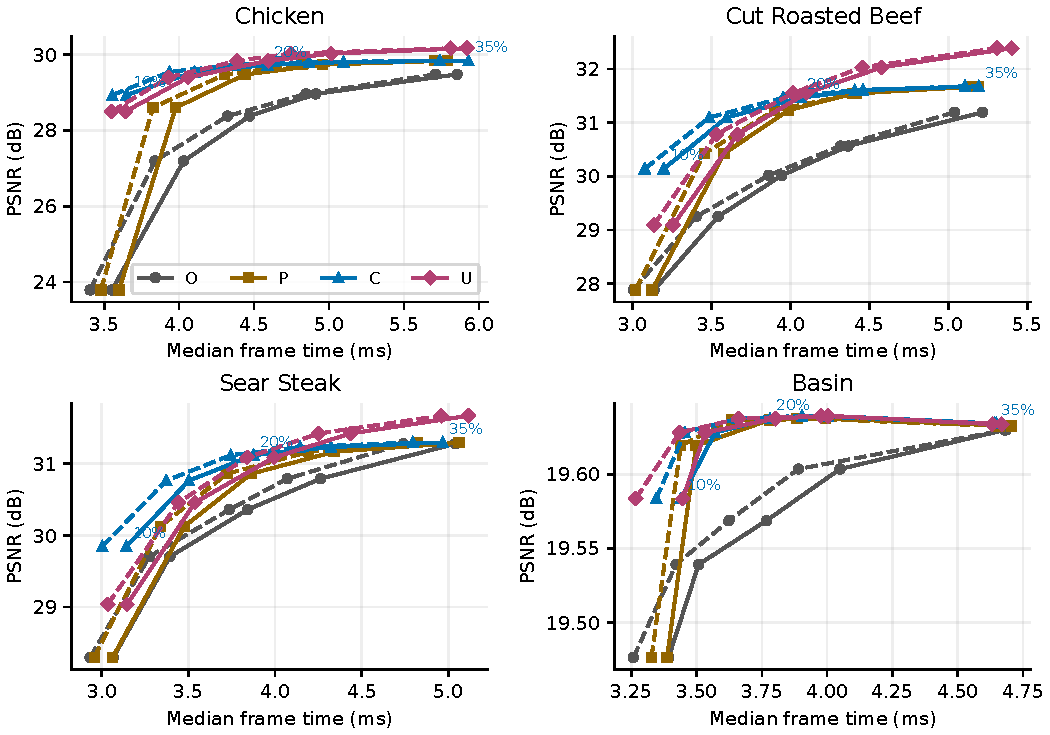
\includegraphics[width=.86\textwidth]{results_assets/cost.pdf}
\caption{Cold PSNR versus measured resident-render latency. Each point combines mean PSNR and the median of the three source-level p50 frame times for the same arm and retained count. Solid lines show dynamic gathering and dashed lines show compact subsets. Lines connect observations in budget order. Dynamic C is annotated at 10, 20, and 35\%.}
\label{fig:cost}
\end{figure*}

\begin{table*}[t]
\centering\small
\caption{Fine-tuned 15\% compact frame latency. Each entry is the median across three sources of the displayed statistic. The last two columns first form the corresponding latency ratio to O within each source.}
\label{tab:timing}
\begin{tabular}{lccccc}
\hline
Scene & Arm & p50 (ms) & p95 (ms) & p50/O & p95/O \\
\hline
\resultrows{results_assets/timing.tex}
\hline
\end{tabular}
\end{table*}

\begin{table*}[t]
\centering\small
\caption{Separately instrumented cold dynamic stages at 15\% for O, C, and U. Entries are medians across sources of stage medians in milliseconds.}
\label{tab:profile}
\begin{tabular}{lcccc}
\hline
Scene & Arm & Gather & Deformation & Rasterization \\
\hline
\resultrows{results_assets/profile.tex}
\hline
\end{tabular}
\end{table*}
